
\begin{IEEEbiography}[{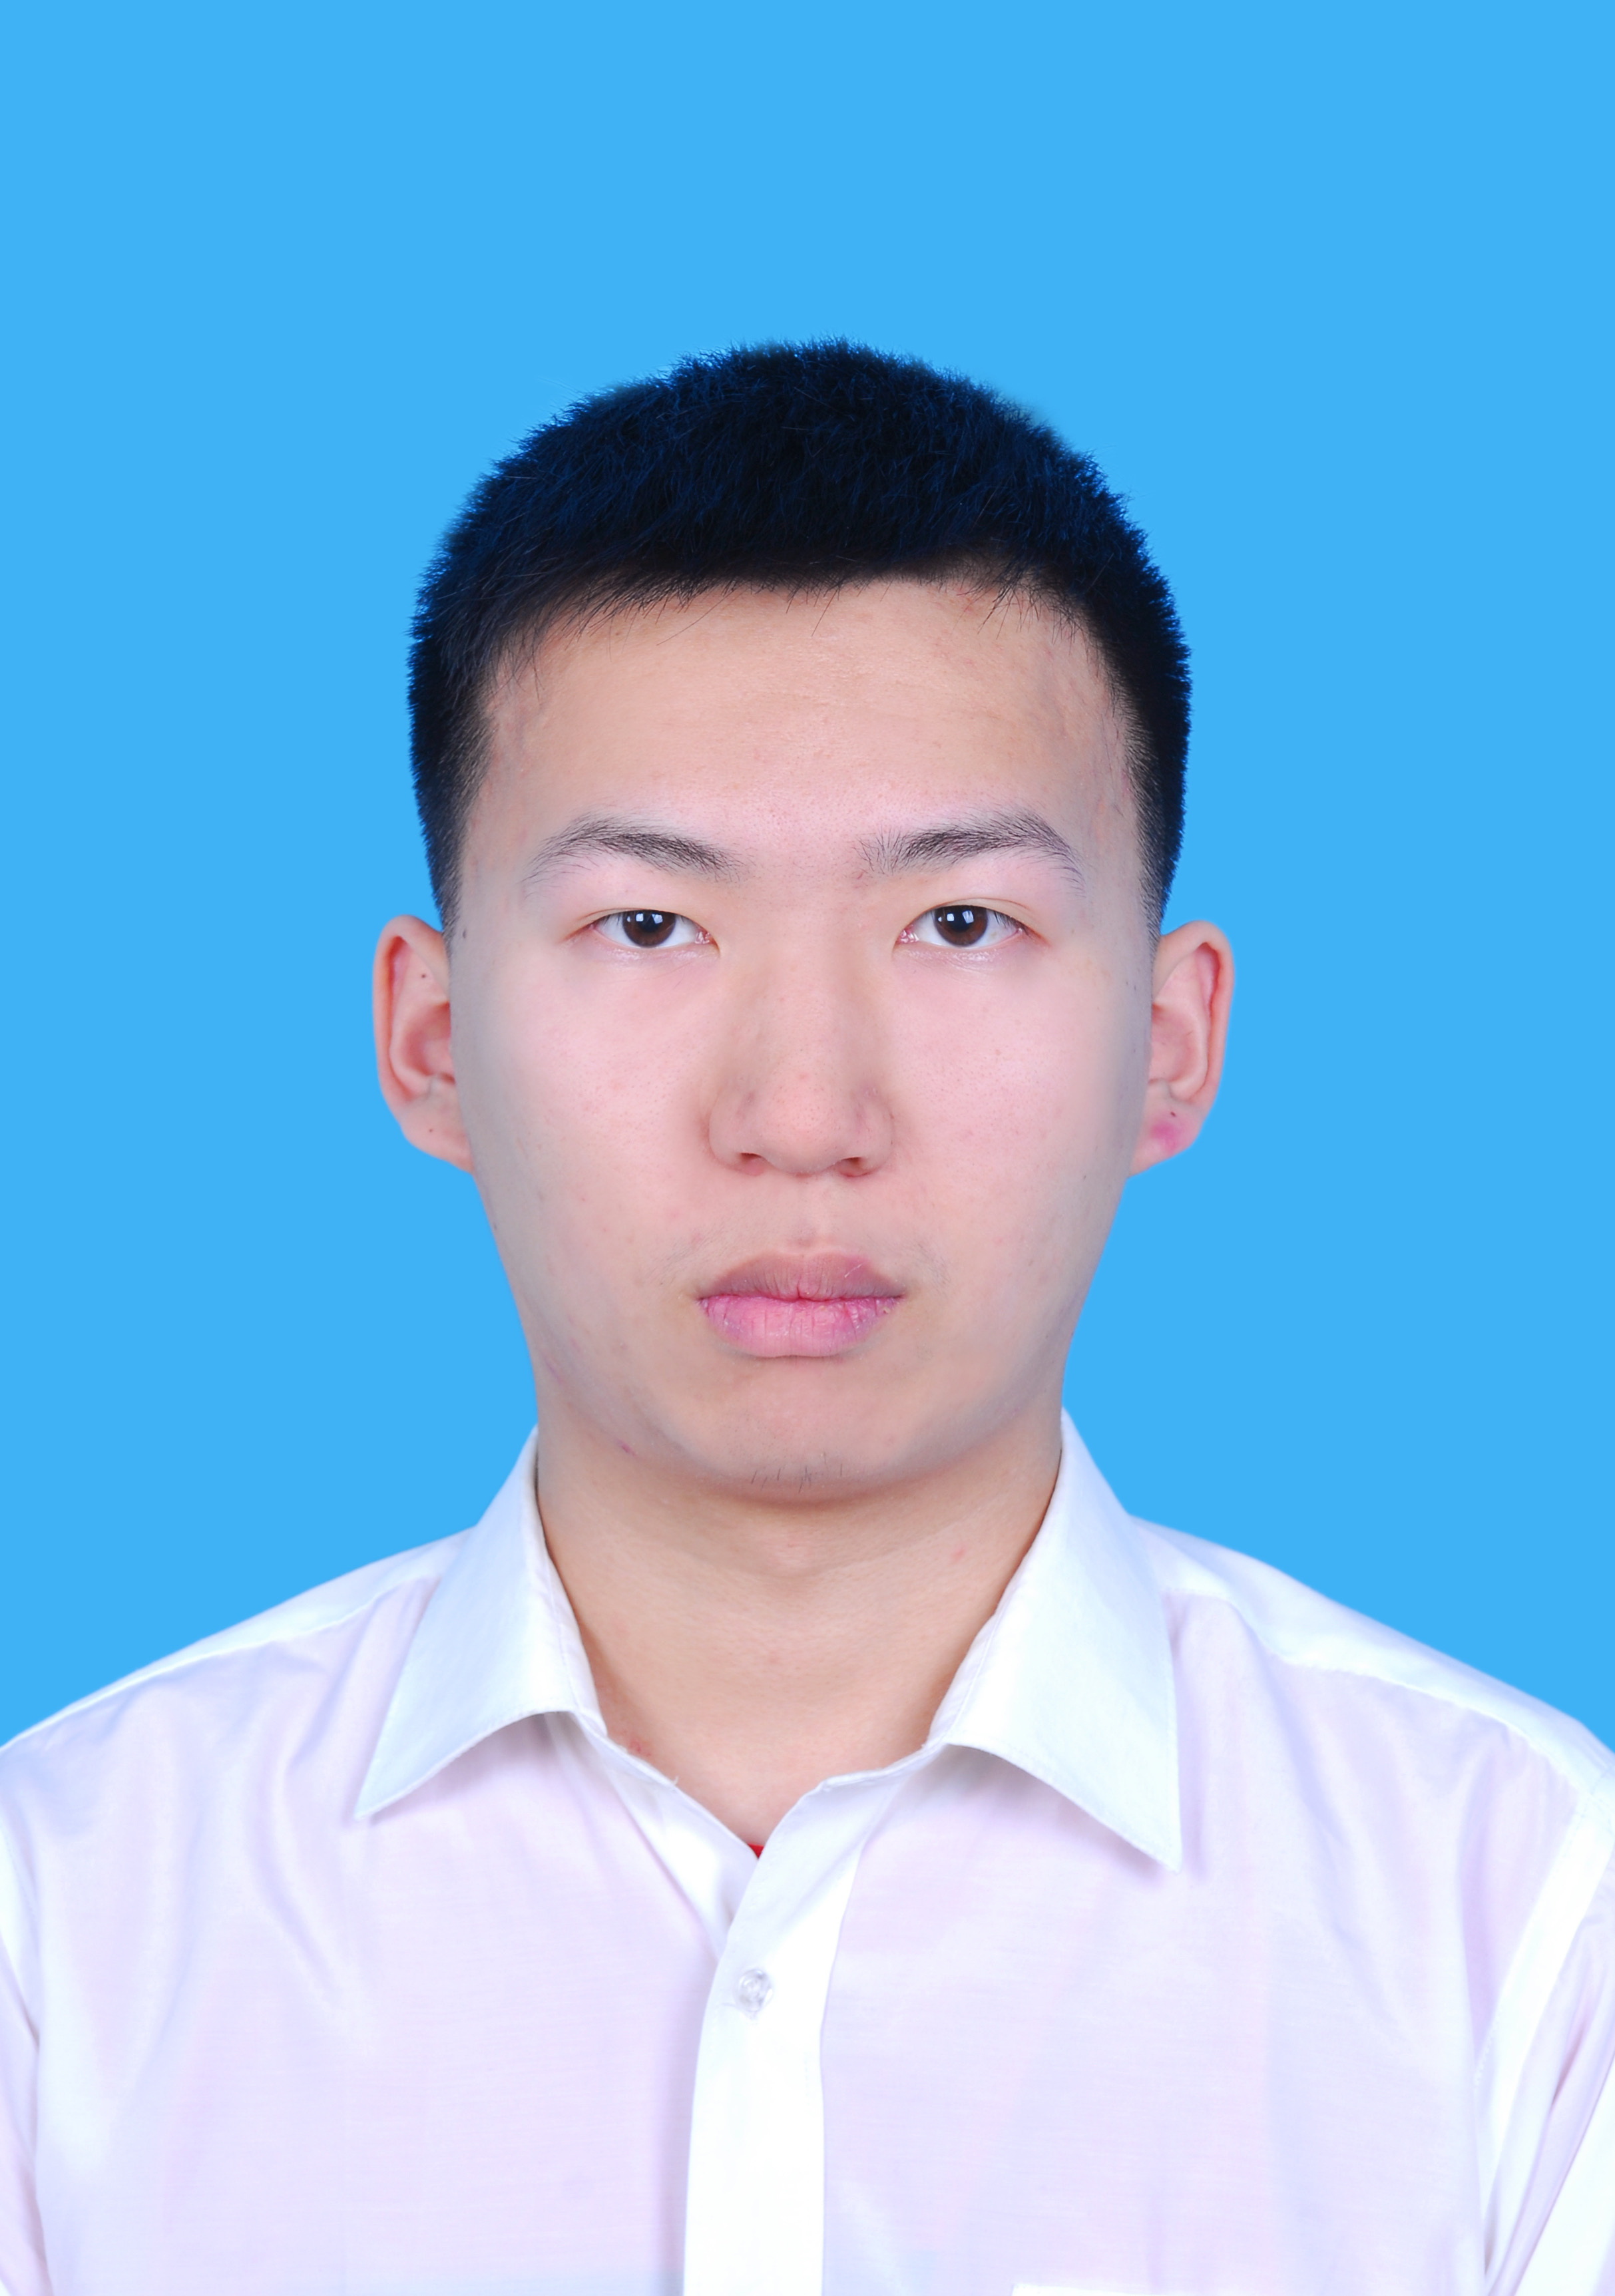
\includegraphics[height=1.25in,clip,keepaspectratio]{figs/bio/shidong_cao.png}}]{Shidong Cao}
received the BE degree from Beijing University of Posts and Telecommunications, China. He is currently working toward the MS degree with Zhejiang University - University of Illinois Urbana-Champaign Institute, Zhejiang University. His research interests include machine learning and computer vision.
\end{IEEEbiography}

\begin{IEEEbiography}[{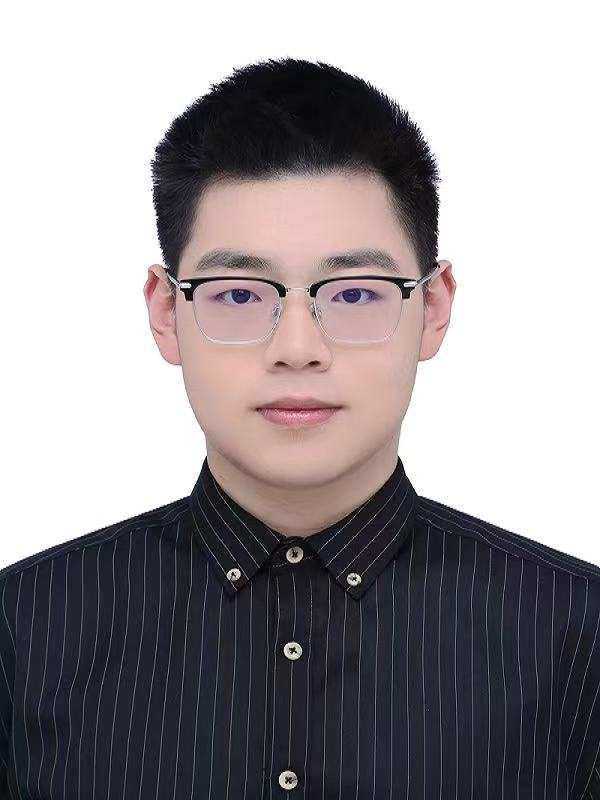
\includegraphics[height=1.25in,clip,keepaspectratio]{figs/bio/zhonghan_zhao.jpg}}]{Zhonghan Zhao}
received a B.S. degree from the Communication University of China. He is currently working toward a Ph.D. degree with Zhejiang University - University of Illinois Urbana-Champaign Institute, Zhejiang University. His research interests include machine learning, reinforcement learning, computer vision, and embodied agents.
\end{IEEEbiography}


\begin{IEEEbiography}[{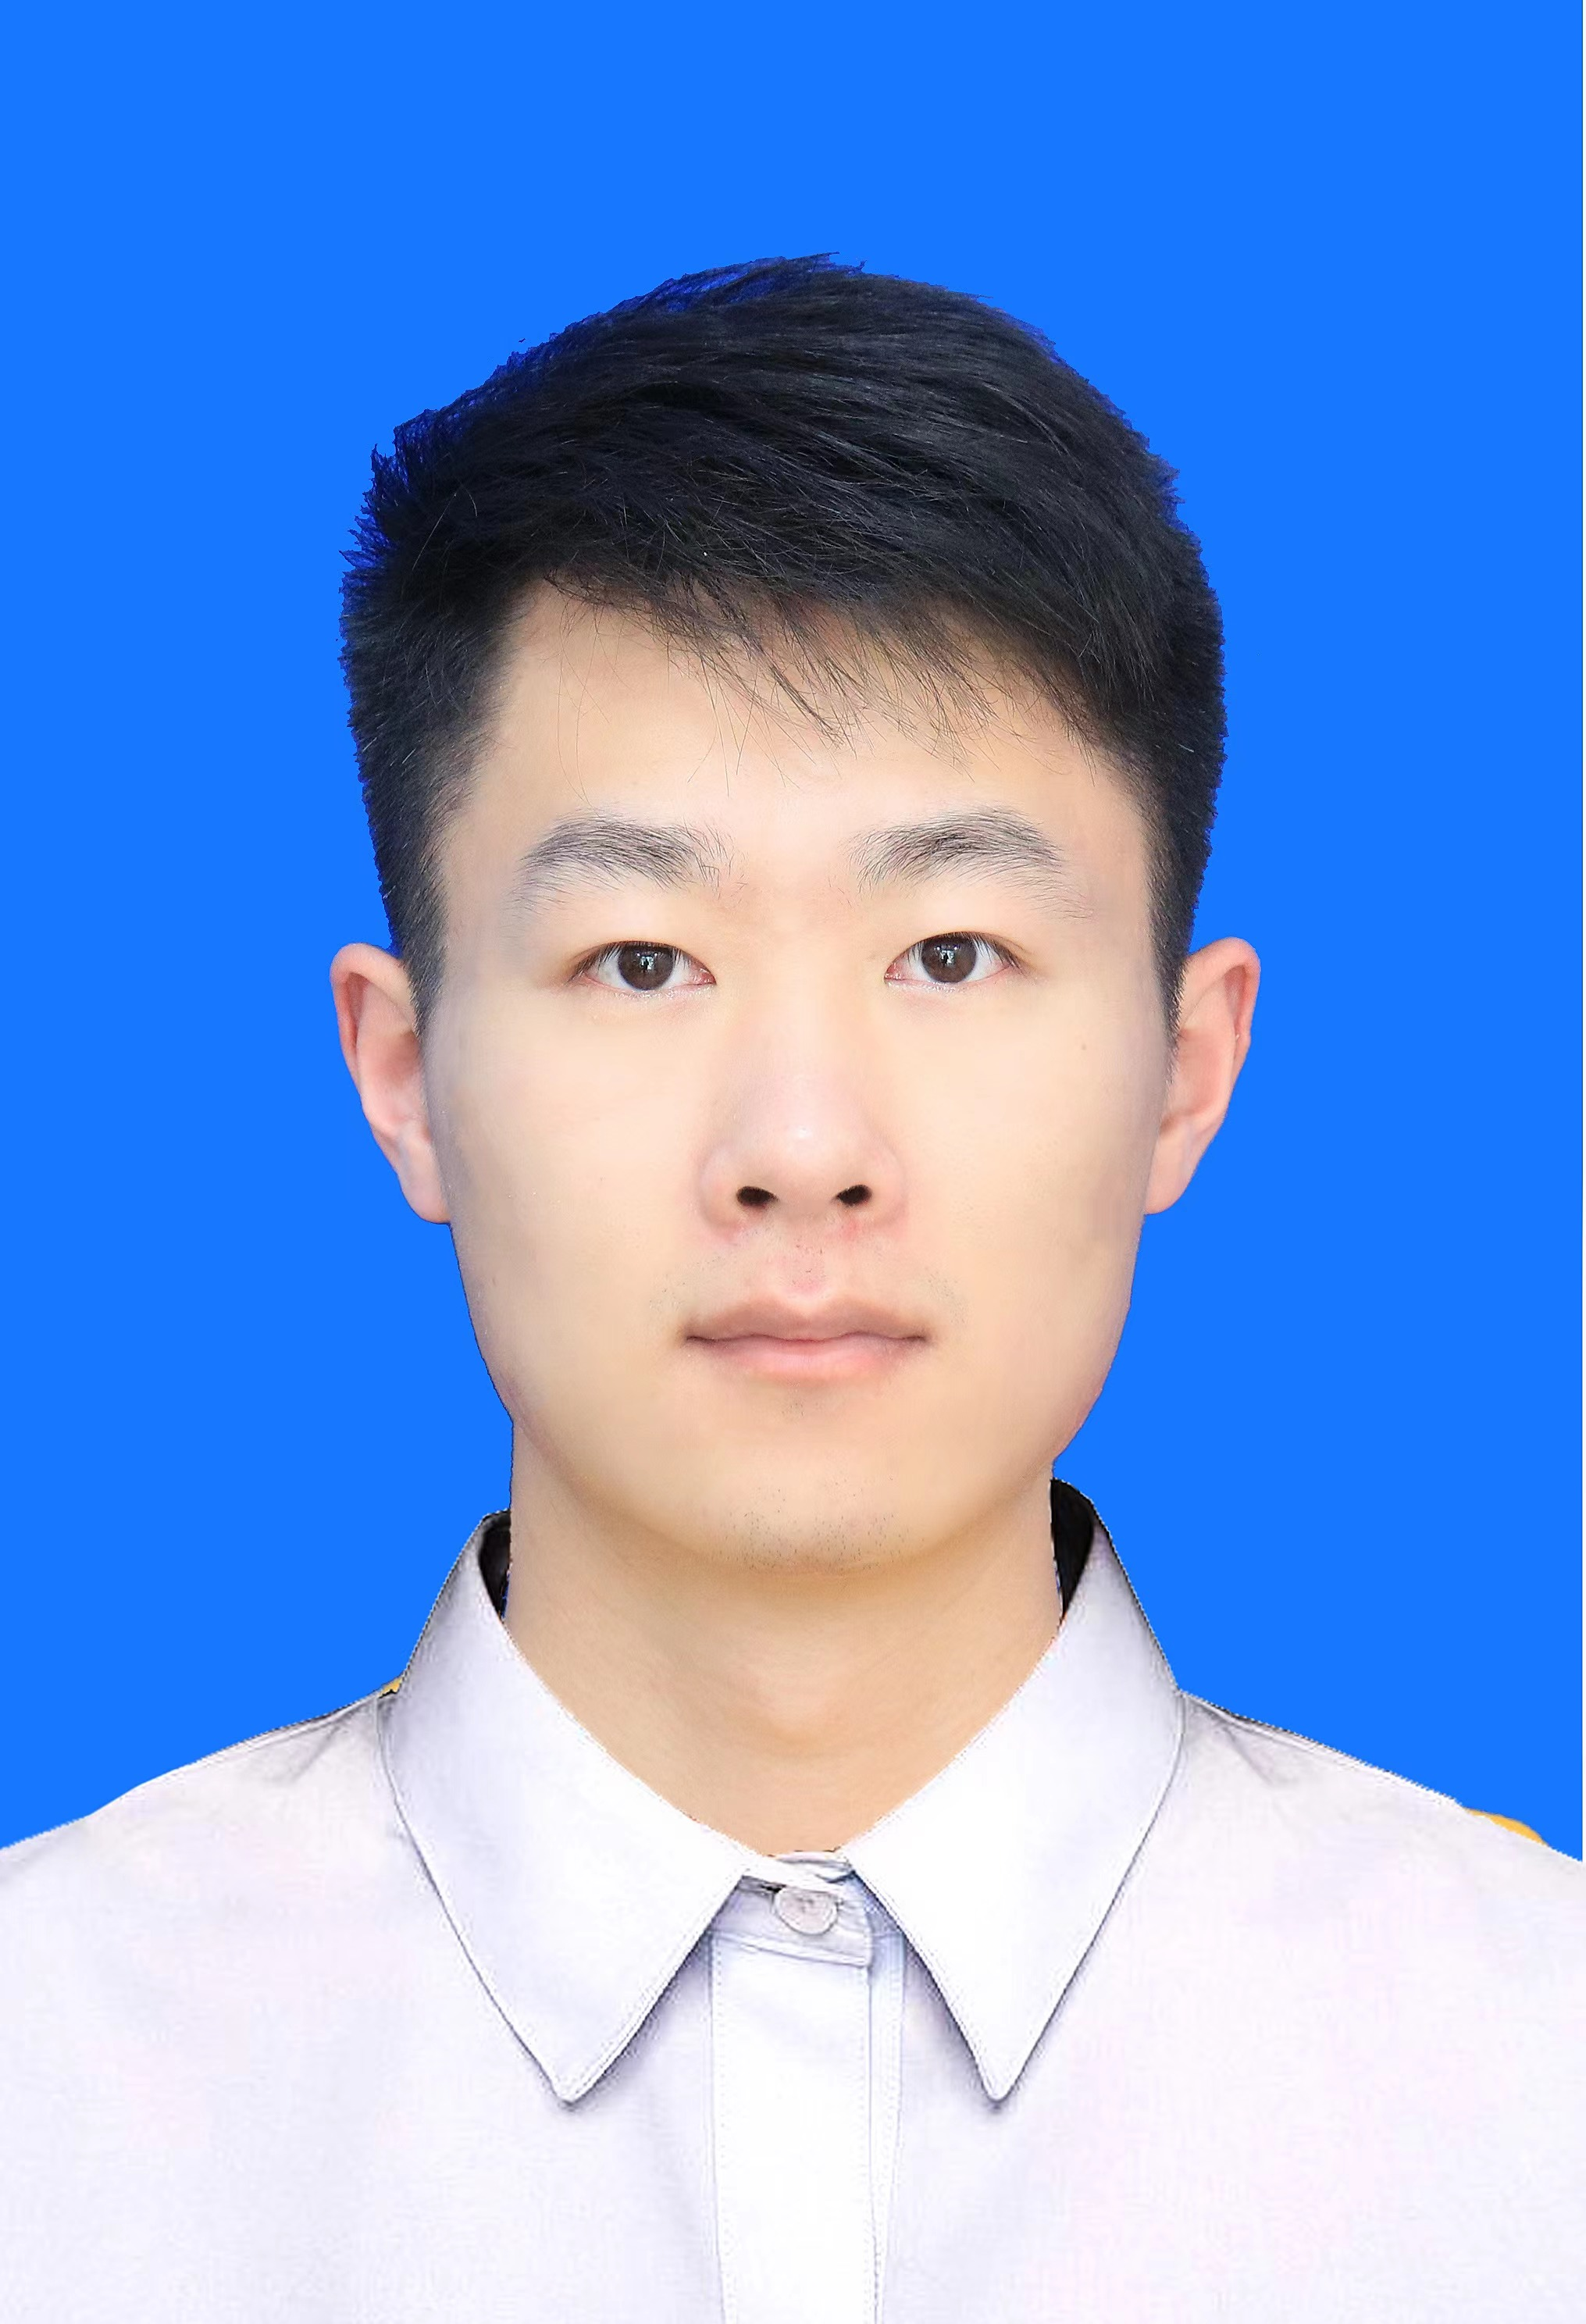
\includegraphics[height=1.25in,clip,keepaspectratio]{figs/bio/shengyu_hao.jpg}}]{Shengyu Hao}
received the MS degree from Beijing University of Posts and Telecommunications, China. He is currently working toward the PhD degree with Zhejiang University - University of Illinois Urbana-Champaign Institute, Zhejiang University. His research interests include machine learning and computer vision.
\end{IEEEbiography}

\begin{IEEEbiography}[{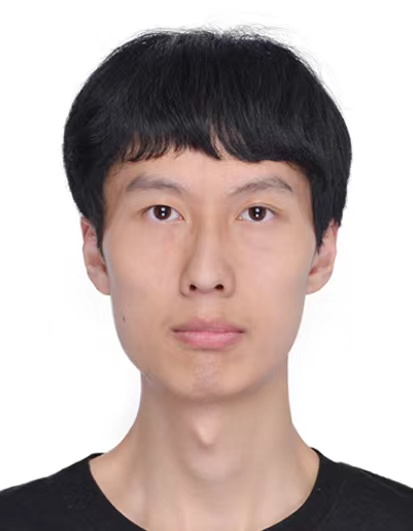
\includegraphics[height=1.25in,clip,keepaspectratio]{figs/bio/wenhao_chai.jpg}}]{Wenhao Chai}
received the BE degree from Zhejiang University, China. He is currently working toward the Master degree with University of Washington. His research interests include generative models and multi-modality learning.
\end{IEEEbiography}

\begin{IEEEbiography}[{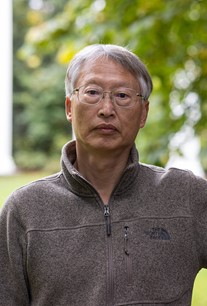
\includegraphics[height=1.25in,keepaspectratio]{figs/bio/Jenq-NengHwang.jpg}}]{Dr. Jenq-Neng Hwang}
received the B.S. and M.S. degrees in electrical engineering from the National Taiwan University, Taipei, Taiwan, in 1981 and 1983 separately. He then received his Ph.D. degree from the University of Southern California. In the summer of 1989, Dr. Hwang joined the Department of Electrical and Computer Engineering (ECE) of the University of Washington in Seattle, where he has been promoted to Full Professor since 1999. He is the Director of the Information Processing Lab. (IPL), which has won several AI City Challenges and BMTT Tracking awards in recent years. Dr. Hwang served as associate editor for IEEE T-SP, T-NN and T-CSVT, T-IP, and Signal Processing Magazine (SPM). He was the General Co-Chair of the 2021 IEEE World AI IoT Congress and the program Co-Chairs of IEEE ICME 2016, ICASSP 1998, and ISCAS 2009. Dr. Hwang is a fellow of IEEE since 2001.
\end{IEEEbiography}



\begin{IEEEbiography}[{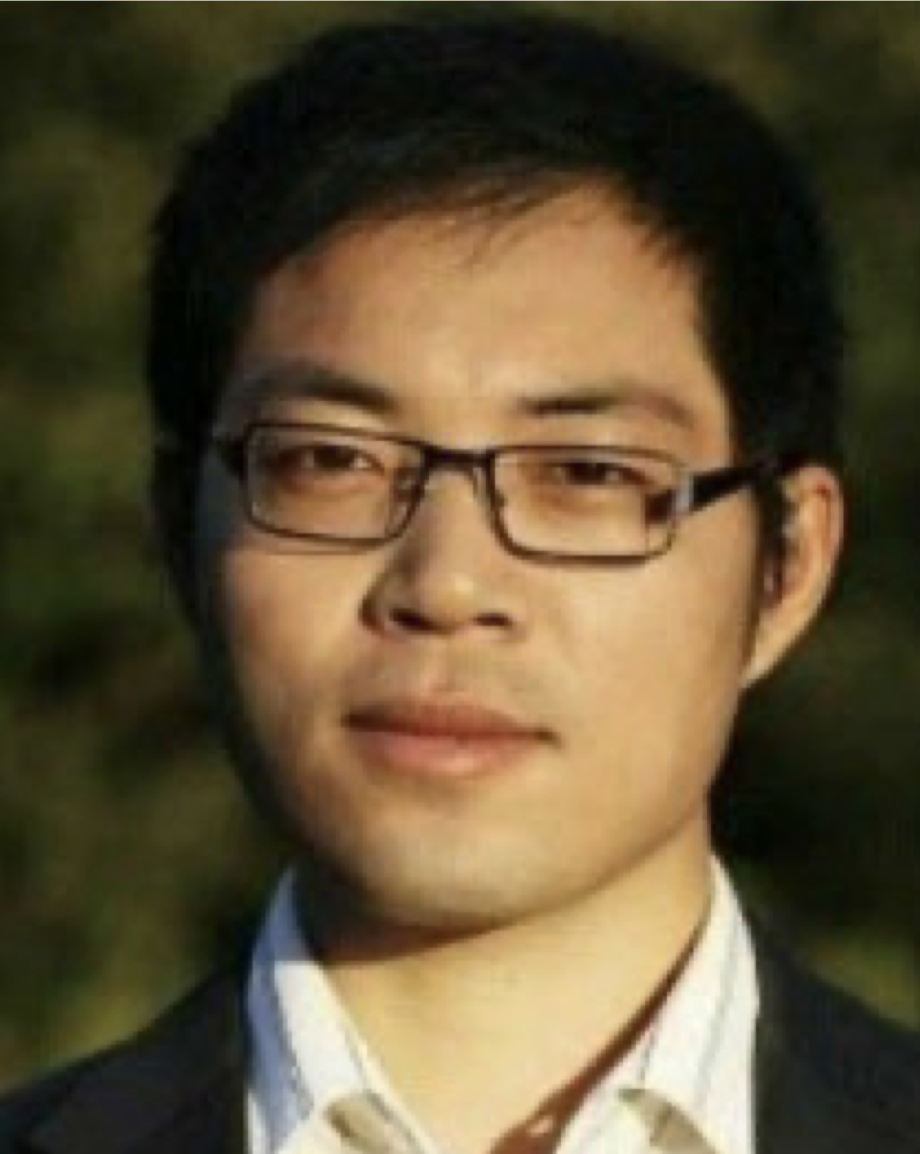
\includegraphics[width=1in,height=1.25in,clip,keepaspectratio]{figs/bio/hongwei_wang.png}}]{Dr. Hongwei Wang}
received the B.S. degree in information technology and instrumentation from Zhejiang University, Hangzhou, China, in 2004, the M.S. degree in control science and engineering from Tsinghua University, Beijing, China, in 2007, and the Ph.D. degree in design knowledge retrieval from the University of Cambridge, Cambridge, U.K., in 2010. From 2011 to 2018, he was a Lecturer and then a Senior Lecturer in engineering design with the University of Portsmouth, Portsmouth, U.K. He is currently a tenured Professor with Zhejiang University and the University of Illinois at Urbana–Champaign Joint Institute, Haining, China. His research interests include knowledge engineering, industrial knowledge graphs, intelligent and collaborative systems, and data-driven fault diagnosis. His research in these areas has been published in over 120 peer-reviewed papers in well-established journals and international conferences.
\end{IEEEbiography}


\begin{IEEEbiography}[{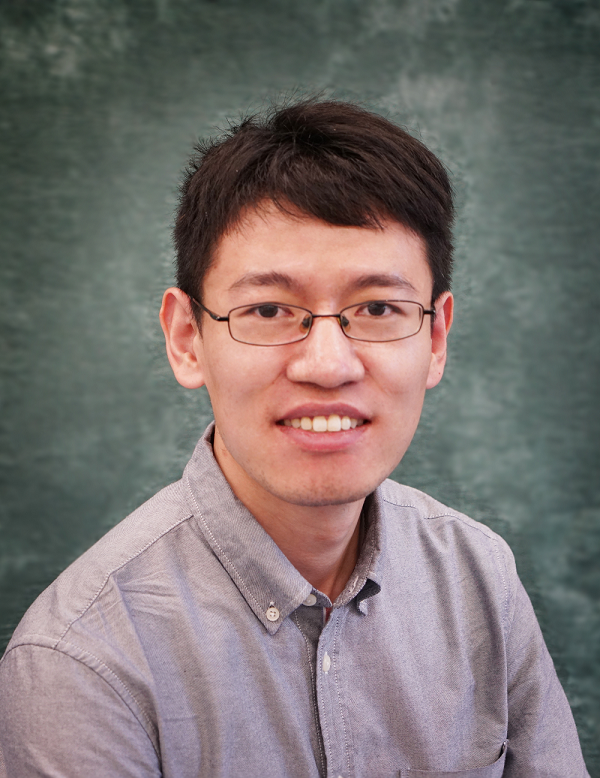
\includegraphics[width=1in,height=1.25in,clip,keepaspectratio]{figs/bio/gaoang_wang.png}}]{Dr. Gaoang Wang}
joined the international campus of Zhejiang University as an Assistant Professor in September 2020. He is also an Adjunct Assistant Professor at UIUC. Gaoang Wang received a B.S. degree at Fudan University in 2013, a M.S. degree at the University of Wisconsin-Madison in 2015, and a Ph.D. degree from the Information Processing Laboratory of the Electrical and Computer Engineering department at the University of Washington in 2019. After that, he joined Megvii US office in July 2019 as a research scientist working on multi-frame fusion. He then joined Wyze Labs in November 2019 working on deep neural network design for edge-cloud collaboration. His research interests are computer vision, machine learning, artificial intelligence, including multi-object tracking, representation learning, and active learning. Gaoang Wang published papers in many renowned journals and conferences, including IEEE T-IP, IEEE T-MM, IEEE T-CSVT, IEEE T-VT, CVPR, ICCV, ECCV, ACM MM, IJCAI.
\end{IEEEbiography}
